\documentclass[preprint,5p]{elsarticle}
\usepackage{graphicx}
\usepackage{dcolumn}
\usepackage{bm}  
\usepackage{amssymb}  
\usepackage{hyperref}
\providecommand{\keywords}[1]{\textbf{\textit{Index terms---}} #1}
\hypersetup{colorlinks=true, urlcolor=blue, citecolor=blue}
\usepackage[displaymath]{lineno}

\linenumbers

\title{\vspace{-15mm}\fontsize{24pt}{10pt}\selectfont\textbf{Rate capability 
and magnetic field tolerance measurements of fast timing microchannel plate 
photodetectors}}
\input author_list.tex  
\date{\today}
\begin{document}


\begin{abstract}
Microchannel plate photodetectors provide both picosecond time resolution and 
sub-millimeter position resolution, they are attractive sensors for particle 
identification detectors of future US Electron Ion Collider. We have tested the 
rate capability and magnetic field tolerance of 6$\times$6 cm$^{2}$ 
microchannel plate photodetectors fabricated at Argonne National Laboratory.  
The microchannel plate photodetector is designed of low-cost all-glass vacuum 
package with a chevron pair stack of ``next generation" microchannel plates 
functionalized by atomic layer deposition. The rate capability test was 
performed with Fermilab 120 GeV primary proton beam, and the magnetic field 
tolerance test was performed on a solenoid magnetic facility with tunable 
magnetic field strength up to 4 Tesla. The gain of measured microchannel plate 
photodetector is stable up to 75 kHz/cm$^{2}$, and varies depending on the 
applied magnetic field strength and rotation angle relative to the magnetic 
field direction.
\end{abstract}

\maketitle

\begin{keywords}
   Fast timing, Microchannel plate, Photodetector, Electron Ion Collider, 
   Particle identification detector, Rate capability, Magnetic field, Rotation 
   angle
\end{keywords}


\section{Introduction} \label{sec:level1}
The Electron Ion Collider (EIC) \cite{EIC} has been recommended in the 2015 
Long Range Plan for Nuclear Science \cite{LRP} as the highest priority for a 
new facility construction, with the mapping of the gluon content of nucleons 
and nuclei as the central goal. Several detector concepts are proposed and 
designed at Argonne National Laboratory (ANL), Brookhaven National Laboratory 
(BNL), Thomas Jefferson National Accelerator Facility (JLab) and some other 
institutes, with slightly different layout. For all these EIC detector designs, 
excellent particle identification (PID), especially hadron ($\pi$/$K$/$p$) 
separations over a wide range of momentum, is essential for the detailed 
measurements of several processes, such as the semi-inclusive deep inelastic 
scattering processes. Time-of-flight systems and imaging \u Cerenkov detectors 
(RICH, DIRC) \cite{RICH,RICH2,DRIC} are proposed and studied, calling for large 
area, low cost photon sensors with high spatial resolution, high rate 
capability, radiation tolerance, magnetic field tolerance and picosecond timing 
resolution. 

Microchannel plate (MCP) photodetectors are compact photon sensors, usually 
with an internal chevron pair stack of MCPs, providing both high spatial and 
temporal resolution in a vacuum package. The Large Area Picosecond 
Photodetector (LAPPD$^{TM}$) is the world largest MCP based photodetector with 
an active area of 20$\times$20 cm$^2$ \cite{LAPPD}. It is designed of a modular 
all-glass detector package with the ``next generation" MCPs produced by 
applying resistive and emissive coatings to borosilicate glass capillary array 
(GCA) substrates through atomic layer deposition (ALD) process. The all-glass 
design and low-cost ``next generation" MCPs provide great advantages to reduce 
the LAPPD$^{TM}$ product cost per area compared to other MCP based 
photodetectors currently available. As a collaborator of the LAPPD project 
\cite{LAPPD2}, we have built a MCP photodetector fabrication system 
\cite{LAPPD-ANL} at Argonne National Laboratory to fabricate 6$\times$6 cm$^2$ 
MCP photodetectors with LAPPD design.  The fabricated MCP photodetectors were 
provided to several experiments for early test and adaption of LAPPD detector.  
The MCP photodetector fabrication system also serves as a R{\&}D platform for 
LAPPD package design validation and optimization. Several 6$\times$6 cm$^2$ MCP 
photodetectors with standard LAPPD design were successfully fabricated and 
tested \cite{ANL-MCPs,Wang-MCPs,Wang-MCPs}, exhibiting high gain over 10$^7$, 
overall time resolution of 35 ps and position resolution better than 1 mm.  The 
excellent performance of these 6$\times$6 cm$^2$ MCP photodetectors shows that 
the low-cost LAPPD$^{TM}$ detector is a promising candidate for EIC PID photo 
sensors.  Performance tests of the MCP photodetectors in high rate, high 
radiation damage and high magnetic field environments are required to further 
validate the application of LAPPD$^{TM}$ detectors as EIC PID photo sensors. 

In this paper, we describe the current design of 6$\times$6 cm$^2$ MCP 
photodetectors fabricated at Argonne National Laboratory, report recent results 
on the performance tests of these 6$\times$6 cm$^2$ MCP photodetectors in high 
rate environment and high magnetic field environment. The direction on further 
optimization of the LAPPD$^{TM}$ design for EIC PID application is also 
addressed at the end of this paper.


\section{Design of the MCP-based photodetector assembly} \label{sec_design}
Current design of the 6$\times$6 cm$^2$ MCP photodetector is developed from the 
original LAPPD internal resistor chain design \cite{Wang-MCPs2}, similar to the 
current standard design of commercial LAPPD$^{TM}$ detectors 
\cite{Craven-MCPs}.  Fig.  1 shows a schematic design (not to scale) of current 
MCP-based photodetector assembly and the electrical circuit diagram.  
\begin{figure}[tbp]
\centering 
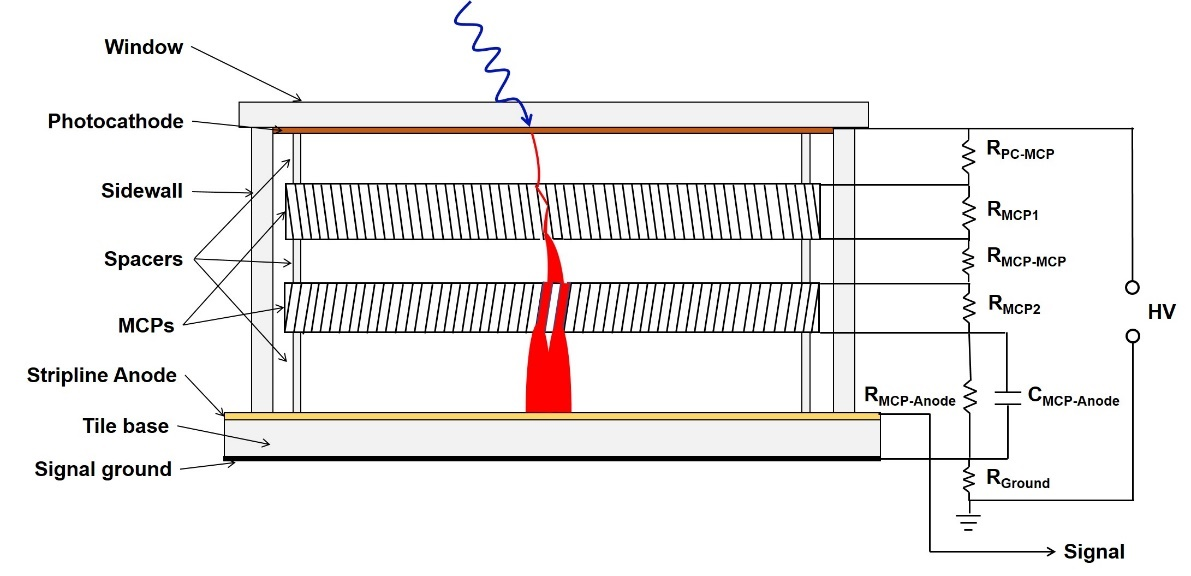
\includegraphics[scale=0.21]{fig/MCPs_design.png}
\caption{Schematic of MCP-based photodetector assembly (not to scale) and the 
   electrical circuit diagram. External connections to the top and bottom 
surfaces of the two MCPs are through ultra-thin metal shims (not shown) to 
special extra strip lines on the tile base. The circuit diagram shows 
connections through side wall in a simplified format.} \label{fig:design}
\end{figure}

The MCP photodetector is an all glass body assembly, consists of glass base 
window, top window, side wall, three grid spacers and two MCPs. The sidewall is 
frit bonded onto the base window, with silver stripline anodes printed, leading 
the signals and high voltage connections to outside. Grid spacers are placed 
between anode and MCPs and top window as insulators to separate these 
components, they also hold these internal components in place in the vacuum 
assembly. Four ultra-thin metal shims are applied at the top and bottom 
surfaces of the two MCPs to lead the electrical connection to external 
connections, detailed circuit connection inside the vacuum package is described 
in reference \cite{Xia-MCPs}. This independent bias-voltage design provides 
advantage of individually controlling and fine tuning of the bias voltage for 
each MCP. Bialkali photocathode is deposited on the inside surface of the top 
window, and an indium seal is made between the top window and the sidewall 
through a low temperature thermo-compression sealing process to form a hermetic 
vacuum detector package. The completed MCP-based photodetector is attached to a 
custom-made circuit board, providing a permanent mount and firm electrical 
connections as shown in Fig. 2. External electrical connections for both signal 
and high voltage are co are inserted into the external resistor connections to 
serve as high voltage divider, ensuring both MCPs work at an independently 
optimized high voltage for best performance. Additional capacitors may also be 
added across the resistor divider for better signal waveform.  

\begin{figure}[tbp]
\centering 
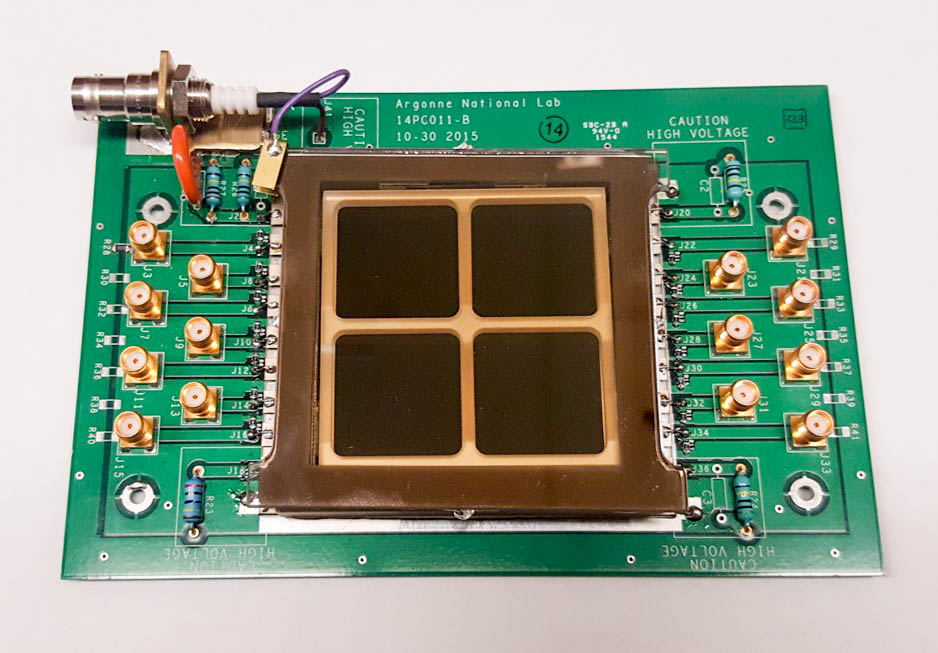
\includegraphics[scale=0.23]{fig/MCPs_assembly.png}
\caption{Completed MCP-based photodetector attached to a circuit board, 
providing firm electrical connections.} \label{fig:MCP_assm}
\end{figure}

The microchannel plates used in the 6$\times$6 cm$^2$ MCP photodetector are 
diced from the ``next generation" large area (20$\times$20 cm$^2$) MCPs 
\cite{LAPPD,Craven-MCPs}, the world largest commercially available MCPs. These 
``next generation" MCPs are produced through a glass drawing process and 
functionalized through atomic layer deposition, completely different from the 
production of traditional leaded glass MCPs. The glass drawing process uses 
borosilicate glass as tube materials, which is considerably less expensive than 
the leaded glass and eliminates the chemical etching process required in 
traditional method, making it much more cost-effective for MCP production.  
Here, we use standard borosilicate glass MCPs with 20 $\mu$m pore size, 60:1 
L/d (pore length to diameter) ratio and 8o bias angle relative to the MCP 
surface normal. The two MCPs are placed as the ``chevron" configuration in the 
vacuum package, which reversed the bias angle to -8$^{\circ}$. 


\section{Rate capability measurement} \label{sec_proton_measurements}
The rate capability of MCP-based photodetectors is one of the most critical 
parameters for applications in high luminosity environment, such as EIC. Due to 
the high resistive layer coating on ALD functionalized MCPs, the current in the 
MCP pores may not flow off fast enough when the MCP-based detector is exposed 
to high particle rates. This effect may cause severe charge saturation, reduce 
the gain of the MCP-based photodetector and limit the detector performance. 
 
We investigated the rate capability of the 6$\times$6 cm$^2$ MCP-based 
photodetectors with 120 GeV/c primary proton beam at the Fermilab Test Beam 
Facility (FTBF). The beam was delivered as a slow spill with a 4 s duration 
once per minute with a maximum intensity of $~$ 10$^5$ particles per spill.  
The beam shape is circular with a diameter of 6 mm and a gaussian density 
profile. The beam intensity was close to a constant during each spill period.  
On the beamline, the 120 GeV/c incident proton beam was monitored by an 
upstream multiwire proportional counter to see the beam profile. Three plastic 
scintillators in coincidence were used as a trigger and to count the number of 
incident proton. A light-tight dark box was designed to hold the MCP-based 
photodetector in the beam path with the detector surface facing the beam 
direction. High voltage was applied to the MCPs through external resistor 
voltage divider, and signals from the strip lines were readout through the 
DT5742 desktop digitizer \cite{Digitizer} produced by CAEN (Costruzioni 
Apparecchiature Elettroniche Nucleari S.p.A.) with a sampling rate of 5 GS/s.  
The digitizer is based on the switched capacitor array DRS4 (Domino Ring 
Sampler) chip \cite{DRS} and have 16 analog input channels and 1 additional 
analog input for fast trigger.

During our experiment, the 120 GeV/c proton beam intensity was tuned to vary 
from 500 to 40,000 particles per spill. The beam rate was calculated using the 
number of triggers per spill and was corrected for the size of the beam spot by 
reconstructing the beam profile. The calculated beam rate varies from 3 to 150 
kHz/cm$^2$ corresponding to the monitored beam particle intensity. Fig. 3 shows 
the gain of the MCP-based photodetector measured as a function of the beam 
rate. The measured gain of the investigated detector is stable up to a beam 
flux of 75 kHz/cm$^2$ and still over 10$^7$ when the beam flux reaches 150 
kHz/cm$^2$. Such a high rate capability of the MCP-based photodetector would be 
sufficient for EIC PID detectors, which are expected to work at a rate 
environment of  xxx Hz/cm$^2$.

\begin{figure}[tbp]
\centering 
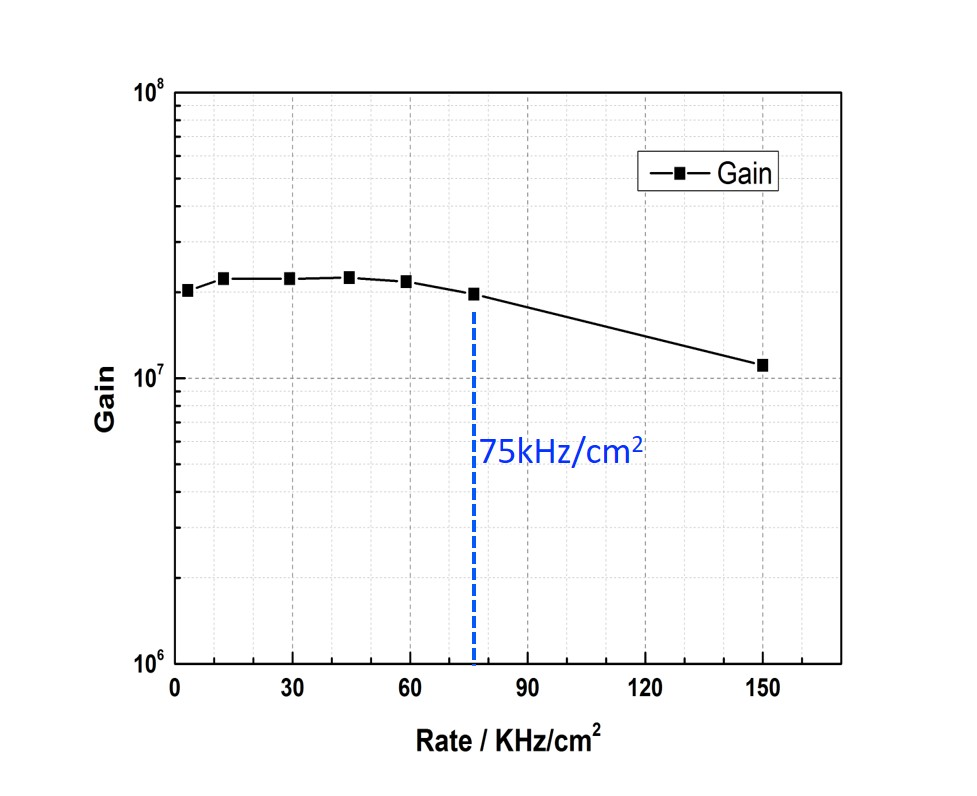
\includegraphics[scale=0.25]{fig/MCPs_gain_proton_beam.png}
\caption{Gain of MCP-based photodetector as a function of the 120 GeV/c proton 
beam flux. The gain of the detector is stable up to beam flux of 75 kHz/cm$^2$, 
and the gain is still over 10$^7$ at 150 kHz/cm$^2$. } 
\label{fig:MCPs_gain_proton_beam}
\end{figure}

\section{Magnetic field tolerance measurement}\label{sec_B_measurement}
In the EIC detectors, solenoid magnet with field strength of ~ 1.5 Tesla are 
proposed. The imaging \u Cerenkov detectors (RICH, DIRC) and time-of-flight 
systems are designed to cover the area of the barrel and end caps for charged 
particle ($\pi$/$K$/$p$) separations. This compact design requires the photo 
sensors working properly in a harsh environment with magnetic field strength up 
to 1.5 Tesla. 

At Argonne National Laboratory, a decommissioned superconducting magnet from a 
magnetic resonance imaging (MRI) scanner was acquired to test instruments for 
the muon g-2 experiment \cite{Magnet}. The magnet provides a large bore with a 
diameter of $~$ 68 cm and a very homogenous field (7 ppb/cm), the magnitude of 
the magnetic field is tunable up to 4 Tesla. We have built a characterization 
system compatible with the solenoid magnet to test the performance of the 
6$\times$6 cm$^2$ MCP-based photodetector in strong magnetic field environment.  
The MCP photodetector was fixed in a custom built non-magnetic, light-tight 
dark box. The dark box was held on a test platform with the detector surface 
normal to the direction of magnetic field. The position of the dark box was 
adjusted so that the center of the MCP photodetector is well aligned with the 
center of the solenoid magnet. A rotation mechanism was also integrated with 
the system, allowing rotation of the MCP-based photodetector with angle 
$\theta$ as shown in Fig. 4 (not to scale). A 405 nm light-emitting diode (LED) 
was used as the light source and introduced to the surface of the MCP 
photodetector through an optical fiber. High voltage was applied to the MCPs 
from a supply with variable voltage control, and signals from the strip lines 
were readout through CAEN DT5742 desktop digitizer.

\begin{figure}[tbp]
\centering 
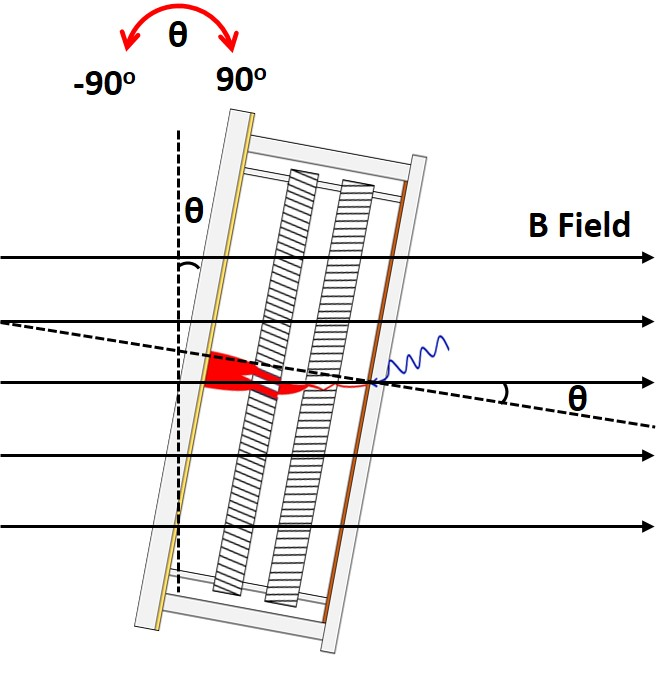
\includegraphics[scale=0.27]{fig/MCPs_theta_rotation.png}
\caption{Schematic of the rotation of MCP-based photodetector with angle 
$\theta$ relative to the magnetic field direction during the measurement.} 
\label{fig:MCPs_theta_rotation}
\end{figure}

\subsection{Magnetic field strength dependence}\label{subsec_HV}
\begin{figure}[tbp]
\hspace{-1.0 cm} 
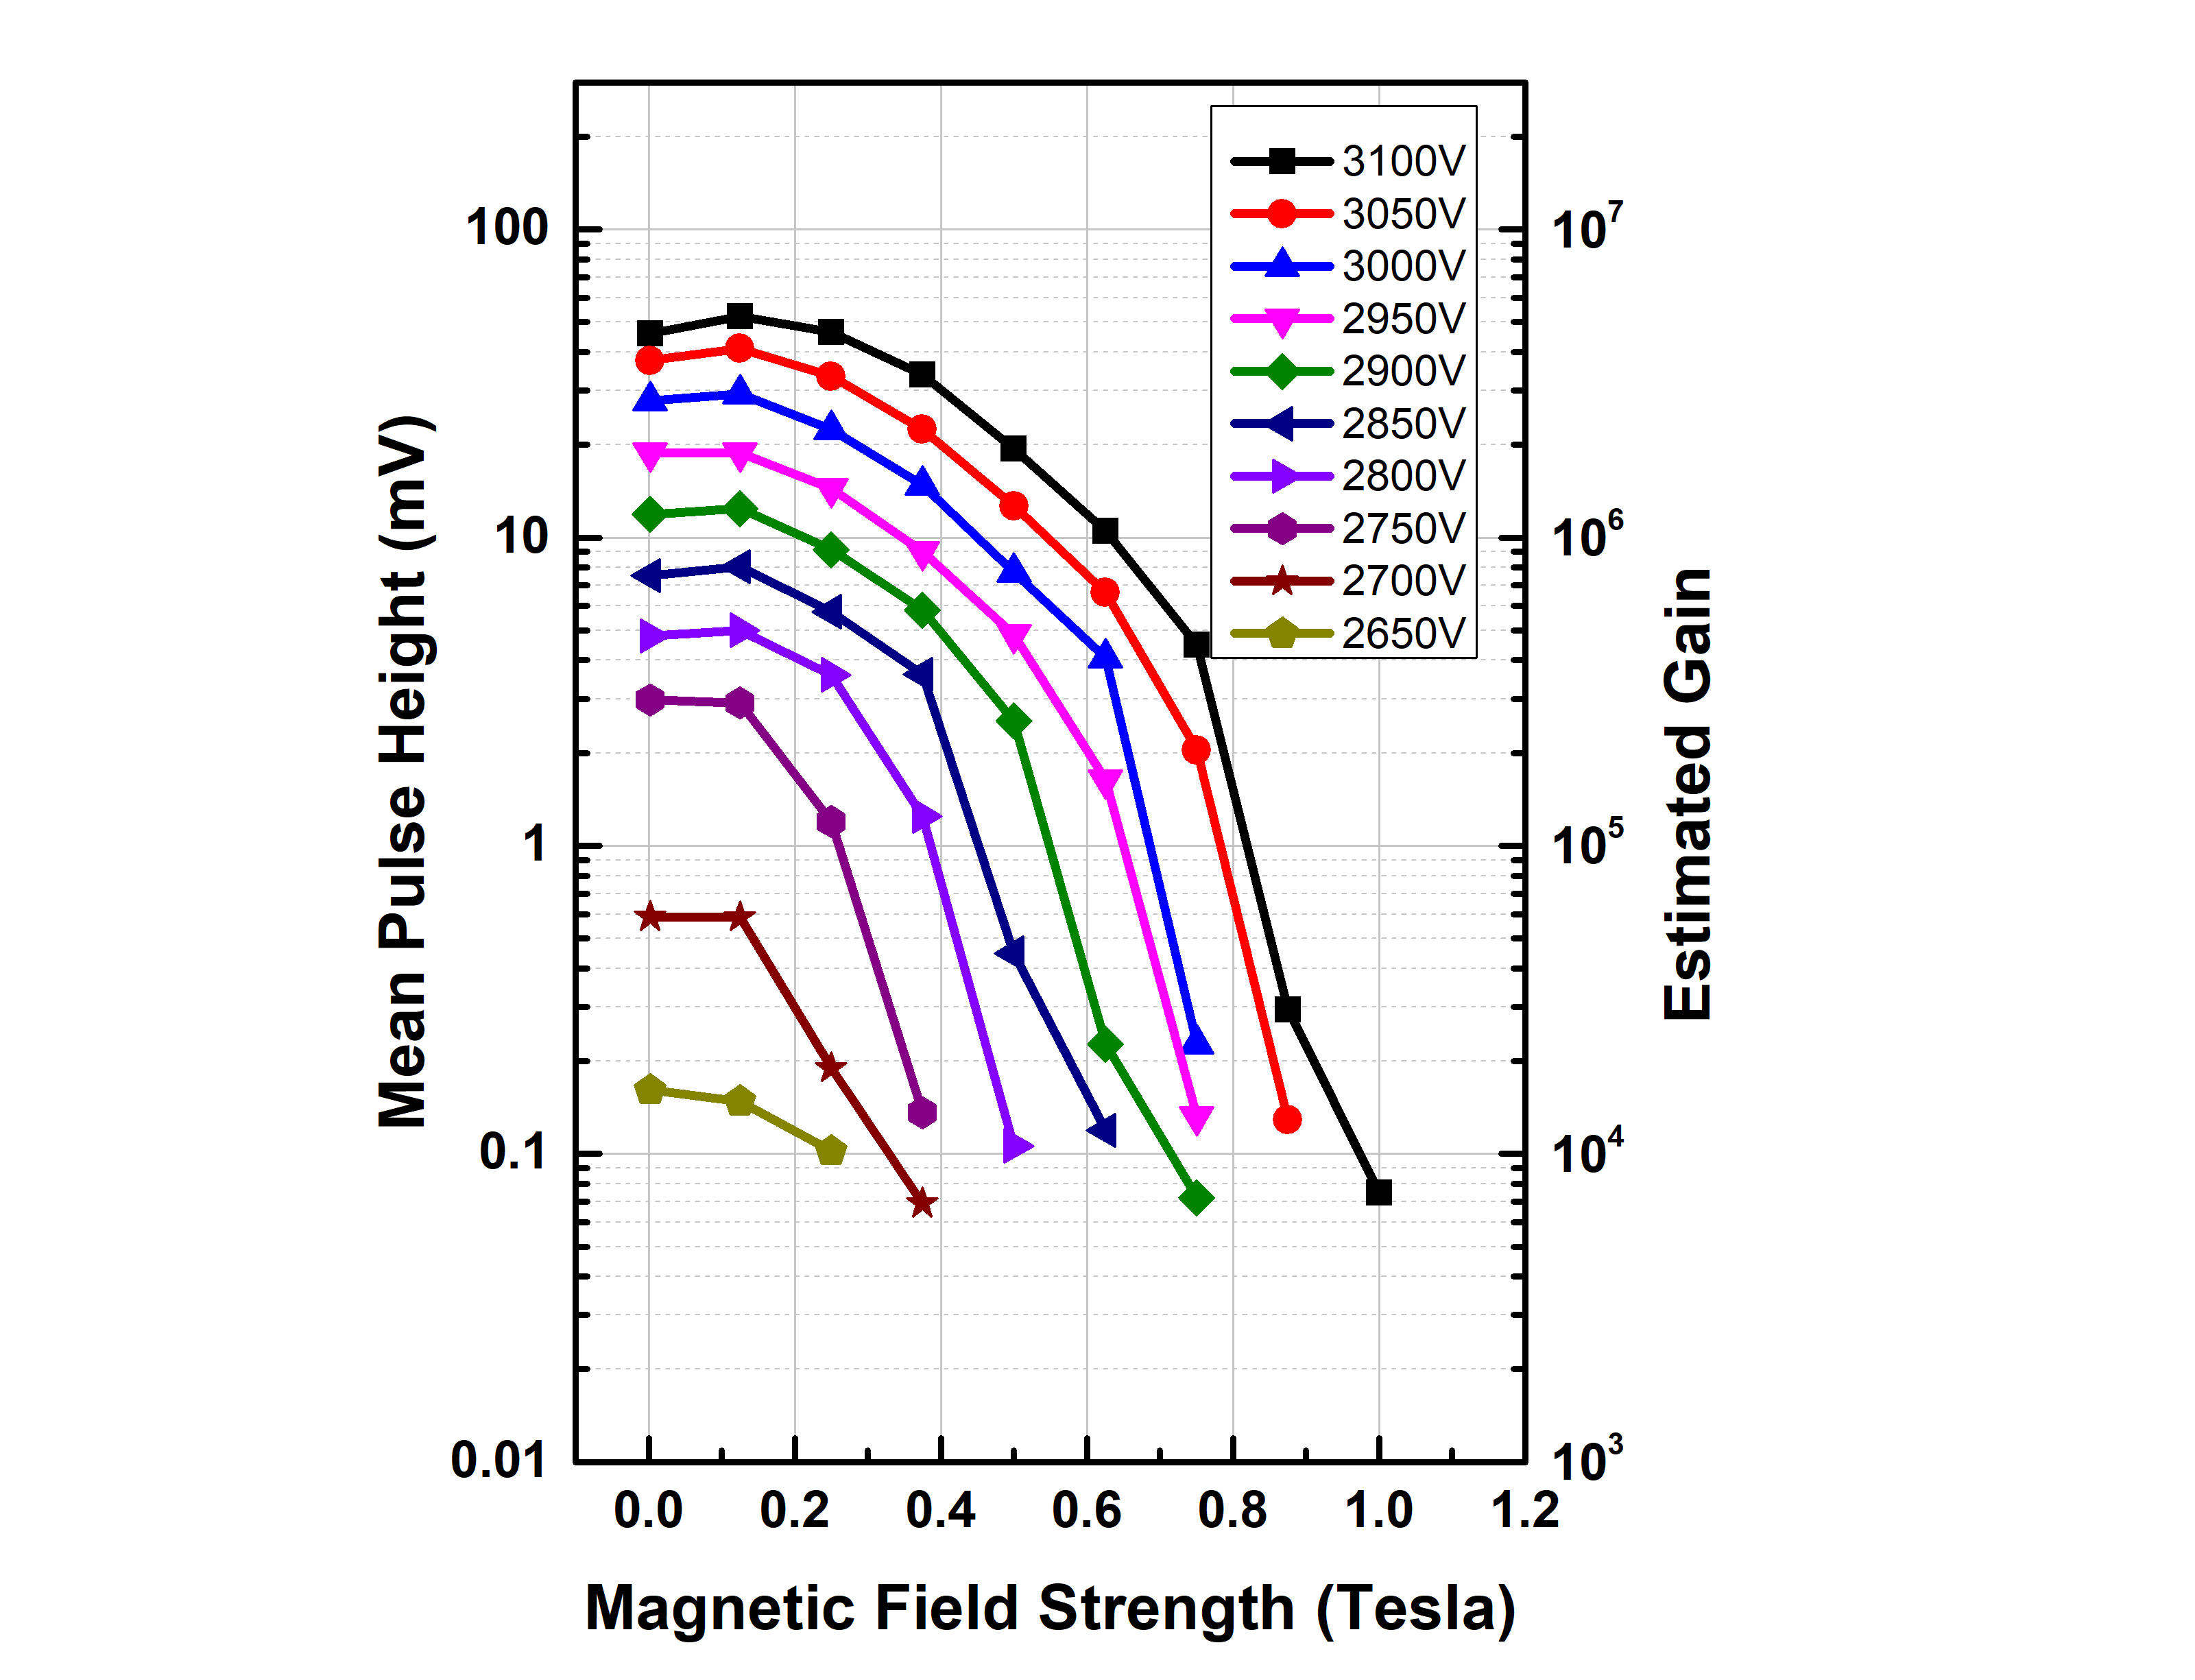
\includegraphics[scale=0.1]{fig/MCPs_gain_B_HV.png}
\caption{Dependence of the MCP-based photodetector gain on the magnetic field 
strength at different bias voltages.} \label{fig:MCPs_gain_B_HV}
\end{figure}

The dependence of the MCP photodetector performance on the magnetic field 
strength was done at rotation angle $\theta$ = 0$^{\circ}$, i.e., the direction 
of the magnetic field is normal to the surface of the MCP-based photodetector.  
We measured the gain of the investigated MCP photodetector in various magnetic 
field environment with different bias voltages, the results are plotted in Fig.  
5. The gain is calculated based on integrated charge in pulse normalized to 
single photoelectron. At a fixed bias high voltage, the gain of MCP 
photodetector increases slightly as the magnetic field strength increases to 
0.2 T, and starts to decrease as the magnetic field strength continues to 
increase, and eventually breaks down at magnetic field strength of $\sim$~0.8 
T.  In the same magnetic field environment, the gain of the MCP photodetector 
increases as the biased high voltage increases. This behavior is similar to our 
previous measurement of the MCP photodetectors without applying magnetic field. 


\subsection{Magnetic field angle dependence}\label{subsec_theta}

\begin{figure}[tbp]
\centering 
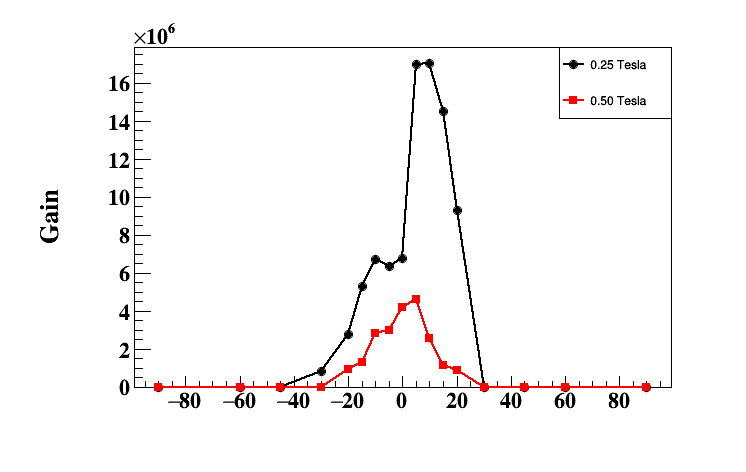
\includegraphics[scale=0.35]{fig/MCPs_gain_theta_B.png}
\caption{Gain of MCP-based photodetector as a function of rotation angle 
   $theta$ relative to the direction of magnetic field. The two peaks around 
-8$^{\circ}$ and 8$^{\circ}$ indicates the effect due to the 8$^{\circ}$ bias 
angle of the MCPs. Note that the intensities of these two peaks are not the 
same due to the different effect from top and bottom MCPs.} 
\label{fig:MCPs_gain_theta_B}
\end{figure}
The performance of MCP-based photodetector at different angle was also studied 
by rotating the MCP photodetector along with angle $\theta$ relative to the 
magnetic field direction, as shown in Fig 5. We fixed the biased high voltage 
at 3000 V on the photodetector and rotated the photodetector from -90$^{\circ}$ 
to 90$^{\circ}$ for a full angle measurement. Fig. 6 shows the gain of MCP 
photodetector measured as a function of the rotation angle $\theta$ at magnetic 
field strength of 0.5 and 0.25 Tesla respectively. The MCP photodetector almost 
does not provide detectable signals when $\theta$~$\leq$~-30$^{\circ}$ or 
$\theta$~$\geq$~30$^{\circ}$. Within - 
30$^{\circ}$~$\leq$~$\theta$~$\leq$~30$^{\circ}$, there are two gain peaks at 
$\theta$ = $\pm$8$^{\circ}$, which are due to the ``chevron" configuration of 
two MCPs inside the photodetector. The gain reaches a maximum when the pore of 
either MCP is well aligned with the magnetic field direction.  Meanwhile, the 
intensities of the two peaks are different, which is due to the different 
effect from the top and bottom MCPs.



\subsection{Design optimization of MCP-based photodetector}\label{subsec_opt}
In EIC experiment, 1.5~Tesla solenoid magnet will be used for tracking charged 
particles. The magnetic field tolerance requirement varies from detector to 
detector depending on their distance and direction to the magnet, and is up to 
1.5 Tesla. From our measurement, the 6$\times$6~cm$^2$ MCP-based photodetector 
has shown a good magnetic field tolerance up to 0.8 Tesla, comparable to that 
of current commercially available MCP-PMTs ($\sim$~1.0~T) with similar pore 
size \cite{MCPs-B}. Here, we must emphasize that the current LAPPD design is 
not optimized yet for magnetic field tolerant applications. The distances 
between the photocathode, MCPs and anode are pretty large in the LAPPD design, 
e.g., spacings between the photocathode and MCPs are 2~mm and the spacing 
between the MCP and anode is 3.2~mm \cite{Wang-MCPs}, these distances should be 
reduced to minimize the electron transit distance. Meanwhile, MCP 
photodetectors with smaller pore size MCPs have shown better magnetic field 
tolerance than the ones with larger pore size MCPs \cite{MCPs-B, Lehmann, 
Ilieva}. A redesign of the current LAPPD configuration with smaller pore size 
(e.g. 10~$\mu$m or even 5~$\mu$m) ``next generation" MCPs and reduced distances 
between the PMT elements would further improve its magnetic field tolerance to 
the required level. 

\section{Conclusions}
We have described the current design of 6$\times$6 cm$^2$ microchannel plate 
photodetectors with ``next generation" MCPs functionalized through atomic layer 
deposition process. The rate capability and magnetic field tolerance of these 
photodetectors were tested at Fermilab 120 GeV proton beam and Argonne 4 Tesla 
magnetic field facility respectively. The photodetectors exhibit stable 
performance up to 75 kHz/cm$^2$ and magnetic field tolerance up to 0.8 Tesla.  
The magnetic field angle dependence was also measured, showing enhanced 
performance at $\pm$8$^{\circ}$ tilt angle due to the original MCP 8$^{\circ}$ 
bias angle. The magnetic field tolerance of these detectors should be further 
improved by applying smaller pore size MCPs and redesign the package with 
reduced distances between the photocathode, MCPs and anode.
 

\input acknowledgment.tex  

\begin{thebibliography}{99}

\bibitem{EIC}
A. Accardi et al., Electron Ion Collider: The Next QCD Frontier, Eur. Phys. J.  
A 52 (2016) 268.

\bibitem{LRP}
A. Aprahamian et al., Reaching for the horizon: The 2015 long range plan for 
nuclear science, 2015. 

\bibitem{RICH}
C.P. Wong et al., Modular focusing ring imaging Cherenkov detector for 
electron-ion collider experiments, Nucl. Instr. and Meth. A 871 (2017) 13.

\bibitem{RICH2}
A. Del Dotto et al., Design and R{\&}D of RICH detectors for EIC experiments, 
   Nucl. Instr. and Meth. A (2017).

\bibitem{DRIC}
G. Kalicy et al., High-performance DIRC detector for the future Electron Ion 
Collider experiment, JINST 11 (2016) C07015.

\bibitem{LAPPD}
   M. Minot et al., Pilot production {\&} commercialization of LAPPD$^{TM}$, 
   Nucl.  Instr.  and Meth. A 787 (2015) 78.

\bibitem{LAPPD2}
B. Adams et al., A brief technical history of the Large-Area Picosecond 
Photodetector (LAPPD) Collaboration, 2016 arXiv:1603.01843.

\bibitem{LAPPD-ANL}
J. Xie et al., Development of a small form-factor (6cm$\times$6 cm) picosecond 
photodetector as a path towards the commercialization of large area devices, 
in: Proceeding of ``The Technology and Instrumentation in Particle Physics 
2014", PoS 2014.

\bibitem{ANL-MCPs}
J. Xie et al., Design and fabrication of prototype 6$\times$6 cm$^2$ 
microchannel plate photodetector with bialkali photocathode for fast timing 
applications, Nucl. Instr. and Meth. A 784 (2015) 242.

\bibitem{Wang-MCPs}
J. Wang et al., Development and testing of cost-effective, 6cm$\times$6cm 
MCP-based photodetectors for fast timing applications, Nucl. Instr. and Meth.  
A 804 (2015) 84.

\bibitem{Wang-MCPs2}
J. Wang et al., Design improvement and bias voltage optimization of glass-body 
microchannel plate picosecond photodetector, IEEE Trans. Nucl. Sci. 64 (2017) 
1871.

\bibitem{Craven-MCPs}
C. Craven et al., Recent advances in Large Area Micro-Channel Plates and 
LAPPD$^{TM}$, Springer Proceedings in Physics (2017).

\bibitem{Xia-MCPs}
L. Xia et al., Systems and methods for forming microchannel plate (MCP) 
photodetector assemblies, U.S. Patent 9704900 B1, July 11, 2017.

\bibitem{Digitizer}
DT5742 desktop digitizer 
\url{http://www.caen.it/jsp/Template2/CaenProd.jsp?parent=14{\&}idmod=651}

\bibitem{DRS}
   DRS chip developed at Paul Scherrer Institut, Switzerland \url{
https://www.psi.ch/drs}

\bibitem{Magnet}
4 Tesla Magnet Facility 
\url{https://www.anl.gov/hep/group/4-tesla-magnet-facility}

\bibitem{MCPs-B}
A. Lehmann et al., Performance studies of microchannel plate PMTs in high 
magnetic fields, Nucl. Instr. and Meth. A 595 (2008) 173.

\bibitem{Lehmann}
A. Lehmann et al., Systematic studies of micro-channel plate PMTs, Nucl.  
Instr. and Meth. A 639 (2011) 144.

\bibitem{Ilieva}
Y. Ilieva et al., MCP-PMT studies at the High-B test facility at Jefferson Lab, 
JINST 11 (2016) C03061.

\end{thebibliography}

\end{document}

